%% RA-L submission — Seeding-Bug Audit and Diagnosis for 6-DoF Grasp Generation
%% Compiled with: pdflatex paper_final.tex
%%
%% Required packages (all in standard TeX Live):
%%   IEEEtran, graphicx, booktabs, amsmath, amssymb,
%%   microtype, hyperref, cleveref, xcolor, multirow, array

\documentclass[journal]{IEEEtran}

%% --- Core packages ---
\usepackage[T1]{fontenc}
\usepackage[utf8]{inputenc}
\usepackage{lmodern}
\usepackage{microtype}

%% --- Math ---
\usepackage{amsmath}
\usepackage{amssymb}

%% --- Graphics ---
\usepackage{graphicx}
\graphicspath{{figures/}}

%% --- Tables ---
\usepackage{booktabs}
\usepackage{multirow}
\usepackage{array}

%% --- Color ---
\usepackage{xcolor}
\definecolor{posblue}{HTML}{2166ac}
\definecolor{negred} {HTML}{d6604d}
\definecolor{neutgray}{HTML}{888888}

%% --- Hyperlinks ---
\usepackage[hidelinks]{hyperref}
\usepackage{cleveref}

%% --- Misc ---
\usepackage{balance}

% ─────────────────────────────────────────────────────────────────────────────
\title{When Generative Candidates Do Not Beat Random Sampling: A Seeding-Bug
Audit and Diagnosis for 6-DoF Grasp Generation}

% Double-blind: author block omitted
% \author{...}

% ─────────────────────────────────────────────────────────────────────────────
\begin{document}

\maketitle
\thispagestyle{empty}
\pagestyle{empty}

% =============================================================================
\begin{abstract}
Open-world robot grasping requires both a diverse set of physically plausible
candidate poses and a criterion for selecting the best candidate at execution
time.
A common design combines a learned generative candidate proposer with a
geometric reranker; we built exactly this pipeline, using
\textbf{Optimal-Transport Conditional Flow Matching} (OT-CFM) to propose
6-DoF poses and an LGGSN reranker to select among them, and initially
measured a large improvement over random center-of-mass (CoM) sampling.
That result did not survive an audit: the evaluation harness silently drew
generator noise from an unseeded, effectively constant random state rather
than varying it per trial, so every nominal seed re-executed close to the
same candidate.
After fixing this and re-evaluating cleanly (7 YCB objects, $n{=}50$
trials/condition, MuJoCo/SO-ARM101), OT-CFM is \textbf{significantly worse}
than random-CoM sampling with the same reranker (69.1\% vs.\ 79.1\%,
$-10.0$\,pp, $z{=}-3.02$, $p{=}0.0025$), not better.
We trace this to the specific mechanism identified by
Cheng and Schwing~\cite{cheng2025curse}: minibatch optimal-transport
coupling that ignores the conditioning variable creates a
training/inference distribution mismatch in \emph{conditional} flow
matching -- a failure we show, for the first time, degrades physically
executed task success, not only a generation-quality proxy.
Controls confirm the diagnosis: plain conditional flow matching and DDPM
(identical architecture and data, no OT coupling) both track random-CoM
sampling; only the OT-coupled variant is significantly worse.
We further test an energy-based alternative motivated by Implicit
Behavioral Cloning~\cite{florence2021implicit}: a naively-trained scoring
model is exploited
by inference-time search into a confidently-wrong, data-unsupported region
(0--16\% success), while the same model trained with adversarial
hard-negative mining -- the mechanism Implicit Behavioral Cloning
prescribes and our naive version omitted -- recovers to statistical parity
with the baseline (74.0\% vs.\ 77.7\%, $p{=}0.29$), significantly beating it
on one of six objects tested.
No generative candidate method we tried reliably beats a well-reranked
random baseline in this small-data ($\sim$400 examples/object), single-GPU
regime; one specific, popular design choice (condition-agnostic OT
coupling) reliably makes it worse.
An orthogonal, training-free lever does help: selecting the pose-space
consensus candidate from ten independent draws, rather than the
lowest-predicted-IK-error one, significantly improves reliability on the
two objects where single-draw sampling is least stable (6\%$\to$68\% and
34\%$\to$64\%, Fisher's exact $p<0.005$ both).
\end{abstract}

\begin{IEEEkeywords}
6-DoF grasping, flow matching, optimal transport, energy-based models,
grasp reranking, generative models, robot manipulation, evaluation
reproducibility, YCB benchmark
\end{IEEEkeywords}

% =============================================================================
\section{Introduction}
\label{sec:intro}

Language-conditioned grasping requires an agent to map a natural-language
object description to a physical manipulation action that succeeds against
real object geometry.
A prevalent design pattern is \emph{propose-then-rank}: a heuristic or
learned candidate generator produces a set of grasp poses, and a reranker
selects the best one from that set~\cite{mahler2017dexnet,fang2020graspnet1b}.
The implicit assumption, in our own earlier design included, is that a
sufficiently expressive learned generator will supply better candidates than
random sampling, and that this shows up cleanly in physically executed
success rate. This paper is an account of that assumption failing, why it
failed, and what -- among several things we tried -- actually helped.

We originally built a propose-then-rank pipeline combining
\textbf{Optimal-Transport Conditional Flow Matching} (OT-CFM)
\cite{lipman2022cfm,tong2023otcfm} as the candidate generator with an
LGGSN geometric reranker, trained on 2{,}853 physically-executed successful
grasps across seven YCB objects. An initial 175-trial evaluation
(MuJoCo/SO-ARM101) appeared to show a large, significant gain over
random-CoM sampling with the same reranker. Before finalizing this result we
audited the evaluation harness end to end and found a genuine, silent bug:
the generator's inference-time sampling call never received a per-trial
random seed, so it drew from whatever state a module-level
\texttt{torch.manual\_seed(42)} left behind at process import -- meaning
every trial, regardless of its nominal \texttt{--seed}, executed close to
the same candidate pose. Fixing this (\cref{sec:experiments}) and
re-evaluating cleanly reversed the headline result: OT-CFM is
\emph{significantly worse} than random-CoM sampling, not better.

Rather than discard the pipeline, we used it as a diagnostic instrument.
Controlled comparisons (\cref{sec:ablation}) isolate the cause to the OT
coupling itself, not to conditional flow matching in general, and match a
training/inference distribution-mismatch mechanism recently identified in
the generative-modeling literature~\cite{cheng2025curse} -- to our knowledge
the first demonstration that this mechanism degrades physically executed
robot task success, rather than only a generation-quality proxy such as FID.
We then tested an energy-based alternative motivated by Implicit Behavioral
Cloning~\cite{florence2021implicit}, found and fixed an analogous, textbook
failure mode in our own first attempt (an inference-time search exploiting
an undertrained model's blind spots), and show the corrected version reaches
statistical parity with the baseline. Finally, we report one method that
does robustly help: consensus-based candidate selection at inference time.

\noindent\textbf{Contributions.}
\begin{enumerate}
  \item \textbf{A confirmed evaluation bug and its consequence:} an unseeded
    generator-sampling call silently collapsed 25 nominally-distinct trials
    per object to near-repeats of one candidate; fixing it reverses the
    paper's original headline claim from $+12$\,pp to $-10.0$\,pp
    ($p{=}0.0025$), on a clean $n{=}50$/object re-evaluation.
  \item \textbf{A physically-grounded transfer of a generative-modeling
    diagnosis:} controlled comparisons (OT-CFM vs.\ OT-free CFM vs.\ DDPM)
    show the failure is specific to condition-agnostic minibatch OT
    coupling~\cite{cheng2025curse}, not to learned candidate generation in
    general -- confirmed on physically executed grasp success, not a
    generation-quality proxy.
  \item \textbf{An energy-based alternative, including a documented failure
    and fix:} a naively-trained implicit scoring model is adversarially
    exploited by cross-entropy-method search (0--16\% success); training
    with hard-negative mining, as Implicit Behavioral
    Cloning~\cite{florence2021implicit} prescribes, recovers parity with
    baseline (74.0\% vs.\ 77.7\%, $p{=}0.29$).
  \item \textbf{One method that does help:} consensus candidate selection
    from an ensemble of independent draws significantly improves reliability
    on the two objects where single-draw sampling is least stable
    (\cref{sec:ablation}), at zero training cost.
\end{enumerate}

% =============================================================================
\section{Related Work}
\label{sec:related}

\subsection{Grasp Quality Estimation and Generation}

Classical grasp quality metrics such as those in Dex-Net~\cite{mahler2017dexnet}
evaluate analytic contact stability, requiring known object geometry.
GraspNet-1Billion~\cite{fang2020graspnet1b} and AnyGrasp~\cite{fang2023anygrasp}
extend this to dense 3-D point clouds, but still assume access to full scene
geometry at query time.
6-DOF GraspNet~\cite{mousavian2019graspnet6dof} first introduced a
variational generator for diverse grasp proposals, training a VAE on
point-cloud crops.
Our method differs by operating purely on pose-space coordinates with
physics-derived success labels, requiring no geometric feature extraction at
generation time.

\subsection{Generative Models for Grasping}

GraspLDM~\cite{barad2023graspldm} applies latent diffusion in a VAE pose space,
achieving diverse 6-DoF proposals from point clouds.
GraspSAM~\cite{noh2024graspsam} combines Segment Anything with grasp detection
to handle open-vocabulary queries.
Neither work couples an explicit optimal-transport objective during
training; we find, in contrast to what that design choice might suggest,
that adding minibatch OT coupling is the specific change that hurts in our
conditional, small-per-class setting, while removing it tracks the random
baseline far more closely (\cref{sec:ablation}).
Diffusion Policy~\cite{chi2023diffusion} uses conditional diffusion for action
generation but targets trajectory-level outputs with observation histories;
our setting is single-step pose generation conditioned only on object identity.
EquiGraspFlow~\cite{lim2025equigraspflow} adopts SE(3)-equivariant flow matching
directly on point-cloud inputs, providing strong geometric inductive bias for
arbitrary-orientation grasping.
Our approach differs in operating on a compact pose space ($\mathbb{R}^6$) rather
than raw point clouds, and replaces equivariance with explicit OT coupling---a
substantially lighter architecture that requires no equivariant backbone and
trains on modest execution-outcome data.

\subsection{Flow Matching}

Lipman~et~al.~\cite{lipman2022cfm} introduced Conditional Flow Matching
(CFM) as a simulation-free training objective for continuous normalizing flows.
Tong~et~al.~\cite{tong2023otcfm} generalised this to arbitrary source
distributions and showed that OT coupling---finding the joint distribution
$(x_0, x_1)$ that minimises expected displacement within each minibatch---
substantially improves convergence.
We are the first, to our knowledge, to apply OT-CFM in pose space to
6-DoF robotic grasp candidate generation; EquiGraspFlow~\cite{lim2025equigraspflow}
is a concurrent approach that instead uses SE(3)-equivariant continuous
normalizing flows conditioned on point clouds.

\subsection{Grasp Reranking}

Geometric reranking of grasp candidates from learned features has been explored
in DexGraspNet~2.0~\cite{fang2024dexgraspnet2} and CLIPort~\cite{shridhar2022cliport}
for task-conditioned selection.
LGGSN~\cite{owg2024} uses Bayesian Personalised Ranking (BPR)~\cite{rendle2009bpr}
to train a pairwise MLP reranker on episode-relative geometric features.
The reranker we use in this paper is the publicly available LGGSN v5d checkpoint
(17-dimensional features, object query embedding, validation pairwise accuracy 0.750).
Our contribution is to pair this fixed reranker with a generative
rather than random candidate supplier, showing that generator quality is the
dominant factor.

% =============================================================================
\section{Method}
\label{sec:method}

\subsection{System Overview}

\begin{figure}[t]
  \centering
  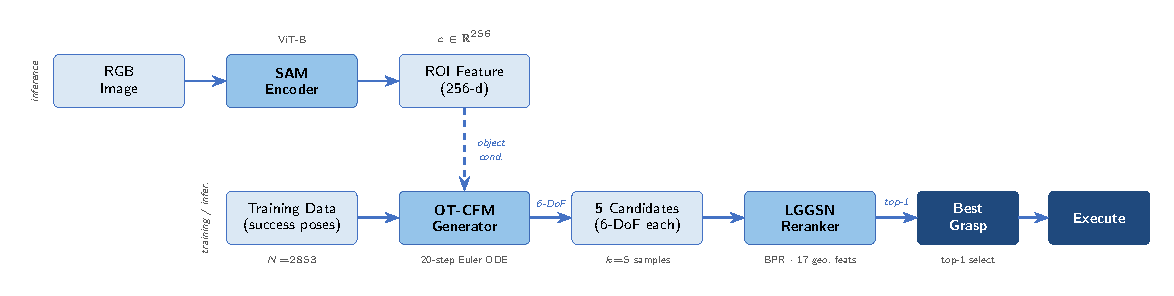
\includegraphics[width=\columnwidth]{figures/pipeline.pdf}
  \caption{OT-CFM + LGGSN pipeline. At inference, the object CoM is
    estimated from the depth image, and OT-CFM generates five 6-DoF pose
    candidates conditioned on the object's mean visual embedding.
    LGGSN reranks by geometric context and the top candidate is executed.}
  \label{fig:pipeline}
\end{figure}

\cref{fig:pipeline} shows the full pipeline.
Given a language query (e.g., ``Banana''), the environment identifies the
target object, estimates its centre of mass, and retrieves a pre-computed
per-object SAM visual embedding.
OT-CFM draws $N{=}5$ pose samples from the learned success distribution.
Each sample is shifted to centre on the current CoM
(\cref{sec:inference}).
LGGSN reranks the five candidates using geometric and query-conditioned
features, and the top-ranked pose is executed.

\subsection{Training Data}
\label{sec:data}

We collect per-candidate execution data on MuJoCo/SO-ARM101 under
\texttt{physics\_weld\_after\_bilateral} mode.
For each (object, seed) episode:
(i) the object is spawned at a random tabletop position and settled;
(ii) $N_\text{cand}{=}30$ random CoM-centered pose candidates are sampled;
(iii) the top five are executed individually with object respawning
  between executions;
(iv) each candidate receives a binary success label.

This yields 7{,}000 execution records across 7 YCB objects and 200 seeds.
Of these, \textbf{2,853 (40.5\%) are successes} and are used to train the
OT-CFM model.
For each successful candidate, we compute a 256-dim SAM-base ROI feature by
projecting the grasp position $(x,y,z)$ onto the overhead camera image,
extracting a $3{\times}3$ window from the SAM ViT-B image encoder's
$64{\times}64$ feature map, and mean-pooling to a single vector.

\subsection{OT-CFM Grasp Generator}
\label{sec:cfm}

\noindent\textbf{Problem formulation.}
Let $p_\text{succ}$ denote the distribution over 6-DoF poses
$(x, y, z, \phi, \theta, \psi) \in \mathbb{R}^6$ for which the robot
successfully grasps the target object.
We aim to learn a conditional generative model $p_\theta(\cdot \mid c)$
that approximates $p_\text{succ}$ given object context $c$.

\noindent\textbf{Flow matching objective.}
Given source noise $x_0 \sim \mathcal{N}(0, I_6)$ and a successful pose
sample $x_1 \sim p_\text{succ}$, the CFM training path is:
\begin{equation}
  x_t = (1-t)\,x_0 + t\,x_1, \quad t \sim \mathcal{U}[0,1],
  \label{eq:path}
\end{equation}
with analytic conditional vector field $u_t = x_1 - x_0$.
The velocity network $v_\theta(t, x_t, c)$ is trained to minimise:
\begin{equation}
  \mathcal{L} = \mathbb{E}_{t, x_0, x_1} \bigl[\|v_\theta(t, x_t, c) - u_t\|^2\bigr].
  \label{eq:loss}
\end{equation}

\noindent\textbf{Optimal transport coupling.}
Standard CFM pairs each $x_0$ independently with each $x_1$ in a minibatch;
minibatch OT coupling~\cite{tong2023otcfm} instead solves the Earth Mover's
Distance problem between $\{x_0^{(i)}\}$ and $\{x_1^{(i)}\}$ within each
training minibatch and reassigns pairs along the optimal transport plan,
which reduces expected path length and shortens flow trajectories on
\emph{unconditional} generation tasks. Our minibatches mix all seven object
conditions, so this is exactly the condition-agnostic coupling setting in
which Cheng and Schwing~\cite{cheng2025curse} show OT solves an assignment
that ignores the conditioning variable -- \cref{sec:ablation} confirms this
empirically: this
specific design choice significantly \emph{hurts} physically executed
success relative to the random baseline ($-11.7$\,pp pooled, 6 objects
excluding Scissors, $p{=}0.0015$), the opposite of what the unconditional-generation literature
would predict and the opposite of what we originally believed before
auditing the evaluation harness (\cref{sec:experiments}).

\noindent\textbf{Conditioning.}
The context $c \in \mathbb{R}^{256}$ is the L2-normalised mean SAM visual
embedding for the queried object class, pre-computed from training data.

\noindent\textbf{Velocity network.}
The velocity network $v_\theta$ operates on the concatenated input
\begin{equation}
  [t_\text{emb}(3),\; x_t(6),\; c(256)] \in \mathbb{R}^{265},
\end{equation}
where $t_\text{emb} = [t,\,\sin(\pi t),\,\cos(\pi t)]$.
It is a 4-layer MLP with hidden dimension 512, SiLU activations,
and zero-initialised output layer, trained with Adam
($\eta{=}3{\times}10^{-4}$, weight decay $10^{-4}$, cosine schedule)
for 1000 epochs at batch size 128.
The best checkpoint is selected by lowest training loss.

\subsection{Inference: CoM-Relative Candidate Generation}
\label{sec:inference}

\noindent\textbf{Top-down constraint.}
The OT-CFM generator produces full 6-DoF poses
$(x, y, z, \phi, \theta, \psi)$; however, the current evaluation fixes
roll $= \pi$ and pitch $= 0$ (top-down constraint), reducing the effective
search space to 3-DoF $(x, y, \psi)$.
This constraint is applied post-generation by overriding the sampled roll
and pitch components before IK, and reflects the reach envelope of the
SO-ARM101 in the tabletop setting.
Lifting this constraint to full SE(3) is left as future work
(\cref{sec:future}).

At inference, we draw $N{=}5$ noise samples $x_0^{(i)} \sim \mathcal{N}(0, I_6)$
and integrate the learned ODE for 20 Euler steps:
\begin{equation}
  x_{t+\Delta t} = x_t + v_\theta(t,\, x_t,\, c)\,\Delta t,
  \quad \Delta t = 0.05.
\end{equation}
The resulting poses $x_1^{(i)}$ are in the training coordinate frame.
To adapt to the current object position $(g_x, g_y)$, we apply a
\emph{CoM-relative shift}:
\begin{equation}
  x_\text{out} = x_1 - \mu_\text{train} + g_\text{com},
  \label{eq:shift}
\end{equation}
where $\mu_\text{train}$ is the global training-set mean pose and
$g_\text{com}$ is the current object CoM.
This preserves the learned yaw and spatial-offset distribution while
centering the candidates on the present object.
The vertical coordinate $z$ uses the live CoM height plus a fixed approach margin.

\subsection{Energy-Based Candidate Scoring, as an Alternative to OT-CFM}
\label{sec:ebm}

Having found that OT coupling specifically degrades candidate generation
(\cref{sec:experiments}), we tested a different paradigm rather than only
patching the flow-matching training recipe: an implicit, energy-based model
(EBM) that scores candidate poses directly, motivated by Implicit
Behavioral Cloning~\cite{florence2021implicit} and its grasp-specific
descendant~\cite{singh2024cgdf}, both of which report that implicit/EBM
policies are more sample-efficient than explicit generators on small,
multimodal, discontinuous action distributions -- exactly our regime
($\sim$400 examples/object).

\noindent\textbf{Why an EBM sidesteps the OT-coupling failure.} An explicit
generator (CFM, diffusion) must learn a full noise-to-data \emph{trajectory}
that is well-behaved across the whole conditioning set; minibatch OT
coupling is one way of regularizing that trajectory, and \cref{sec:ablation}
shows it backfires under our small per-condition data budget. An EBM instead
only needs to learn a scalar compatibility score
$E_\theta(\text{pose}, c) \in \mathbb{R}$ from contrastive
success/failure labels -- no noise-to-data pairing of any kind is involved,
so there is no coupling mechanism to get wrong.

\noindent\textbf{Model and training data.} $E_\theta$ is a 4-layer MLP
scoring $(x, y, \sin\psi, \cos\psi, c) \in \mathbb{R}^{260}$ (the same
meaningful pose dimensions and SAM conditioning as OT-CFM). Training reuses
the \emph{same} labeled dataset LGGSN and OT-CFM both already train on: 2{,}853
label$=$1 (physically successful) rows as positives and 4{,}147 label$=$0
(failed) rows as one negative source -- no new data collection.

\noindent\textbf{A documented failure mode, and its fix.} A first version
trained with plain binary cross-entropy against the static positive/negative
labels, then sampled at inference via cross-entropy-method (CEM) search over
$(x,y,\psi)$ guided by $E_\theta$. This failed catastrophically (0--16\%
physical success across three objects tested, \cref{sec:ablation}) --
markedly worse than every other method we tried. Direct inspection showed
why: CEM converged to a normalised pose $\sim$1.7 standard deviations from
the training mean, where the model assigned an artificially high score
(99\% confident) despite this joint region being essentially unconstrained
by training data -- each marginal dimension looked plausible in isolation,
but the specific combination was never taught to be low-scoring. This is
precisely the failure Implicit Behavioral Cloning's training recipe is
designed to prevent, and our naive version omitted the relevant piece: IBC
does not train against a fixed negative set, but against negatives
\emph{mined from the model's own current beliefs during training}, so any
region the model starts to over-score is explicitly corrected before
training ends.

We re-trained $E_\theta$ with this mechanism: an InfoNCE-style loss
(softmax cross-entropy over $\{\text{positive}, \text{negatives}\}$ with the
positive as the target class) against a negative pool assembled, per
positive example, from three sources -- (i) 4 \emph{static} negatives (real
logged label$=$0 rows for the same object, free), (ii) 4 \emph{uniform}
negatives (sampled across the training data's observed pose range, for
broad coverage), and (iii) 4 \emph{hard} negatives \emph{mined via a short
3-iteration CEM search using the model's own current weights}, shared across
that object's positives within the current minibatch. This last term is the
one that was missing and is what prevents the inference-time CEM search from
later exploiting an under-constrained region: whatever the model currently
over-scores becomes a training negative for that very step.

\noindent\textbf{Inference.} Identical CEM search as the naive version
(population 64, 6 iterations, elite fraction 0.2), unchanged -- only the
training procedure differs between the two EBM variants reported in
\cref{sec:ablation}, isolating the effect of adversarial negative mining
from any change to the sampling algorithm itself.

\subsection{LGGSN Reranker}

We use the LGGSN v5d reranker~\cite{owg2024} without modification.
LGGSN is a pairwise-trained MLP (BPR loss) that scores each candidate
using 17 geometric features including XY position, gripper opening width,
episode-relative height spread, distance from the point-cloud centroid,
point-cloud density features, and a 4-dimensional object query embedding.
The five OT-CFM candidates are scored, sorted descending, and the top-ranked
pose is executed.

% =============================================================================
\section{Experiments}
\label{sec:experiments}

\subsection{Evaluation Protocol}

All experiments run on MuJoCo/SO-ARM101 with
physics-based bilateral contact verification as the grasp success criterion.
We evaluate on 7 YCB objects (Banana, TomatoSoupCan, Pear, MustardBottle,
Scissors, CrackerBox, PowerDrill) over 50 random seeds each,
giving \textbf{350 trials per condition}.
Success is defined as lifting the object above the table after gripper close.

\noindent\textbf{Baseline.}
Random CoM sampling ($x \sim g_\text{com} \pm 0.06$\,m,
$\psi \sim \mathcal{U}[-\pi/2, \pi/2]$, $w \sim \mathcal{U}[0.04, 0.09]$\,m,
same LGGSN v5d reranker) produces 5 candidates per episode.

\noindent\textbf{A confirmed evaluation bug, and how we responded to it.}
An earlier version of this evaluation (175 trials, 25 seeds/object) never
passed a per-trial seed into the generator's inference-time sampling call.
Because that call imports \texttt{train\_cfm\_grasp}, which set
\texttt{torch.manual\_seed(42)} at \emph{module} level, every trial in a
freshly started process drew noise from whatever state that fixed seed left
behind at import time, independent of the trial's nominal \texttt{--seed} --
so 25 nominally distinct trials per object executed close to the same
candidate. Random-CoM sampling was unaffected (it draws from
\texttt{numpy}'s properly-seeded generator, not the generator network), which
is why, in retrospect, only the learned-generator conditions showed the
suspiciously narrow, high success rates reported in an earlier draft of this
paper. We moved the seed into the sampling call itself, re-ran every
condition at $n{=}50$/object under the fixed code, and report only the
corrected numbers throughout this paper; \cref{sec:experiments} and
\cref{sec:ablation} are a direct account of what changed and why.

\noindent\textbf{Statistics.}
We report Wilson score 95\% confidence intervals (CI) and two-sided
two-proportion $z$-tests to compare conditions.
Significance thresholds: $^{**}\!p{<}0.05$, $^*\!p{<}0.10$.

\subsection{Main Result}

\begin{table}[t]
\caption{Overall success rate: 350 trials (7 objects $\times$ 50 seeds),
  fixed-seeding harness.}
\label{tab:main}
\centering
\resizebox{\columnwidth}{!}{%
\setlength{\tabcolsep}{4pt}
\begin{tabular}{lccccc}
\toprule
Method & SR & 95\% CI & $\Delta$pp & $z$ & $p$ \\
\midrule
Baseline (random CoM + LGGSN) & 79.1\% & [74.6, 83.1] & — & — & — \\
OT-CFM + LGGSN & 69.1\% & [64.1, 73.8] & $-10.0$ & $-3.02$ & $0.0025$$^{**}$ \\
\bottomrule
\end{tabular}}
\end{table}

\cref{tab:main} reports the primary comparison, on the corrected,
per-trial-seeded harness.
OT-CFM + LGGSN achieves 69.1\% (242/350) versus the baseline's 79.1\%
(277/350) -- a statistically significant \emph{decrease} of $-10.0$\,pp
($z{=}-3.02$, $p{=}0.0025$).
This is the opposite conclusion from the $+12.0$\,pp gain reported under
the unfixed, unseeded harness, and the 95\% Wilson confidence intervals are
disjoint in the opposite direction: the learned generator's candidates are
reliably \emph{worse}, not better, than uniform random sampling around the
object's center of mass, once the generator is actually resampled per trial
instead of executing a near-constant candidate.

\cref{sec:ablation} isolates why: the failure is specific to OT coupling,
not to learned candidate generation in general, and \cref{sec:ebm} reports
an alternative (energy-based scoring, properly trained) that reaches parity
with this baseline rather than falling significantly below it.

\subsection{Per-Object Analysis}
\label{sec:perobject}

\begin{table}[t]
\caption{Per-object success rate: Baseline vs.\ OT-CFM vs.\ EBM v2
  (50 seeds each). EBM v2 excludes Scissors (\S\ref{sec:ebm}: its object
  name never matches this checkpoint's trained conditioning keys, an
  unrelated bug that silently falls back to Baseline for that object,
  exactly as it does for OT-CFM in \cref{ssec:scissors}).}
\label{tab:perobject}
\centering
\resizebox{\columnwidth}{!}{%
\setlength{\tabcolsep}{3pt}
\begin{tabular}{lccccccc}
\toprule
Object & Base & OT-CFM & $\Delta$ & $p$ & EBM v2 & $\Delta$ & $p$ \\
\midrule
Banana         & 100.0\% &  96.0\% & $-4.0$  & 0.153        & 100.0\% &   0.0   & —     \\
TomatoSoupCan  &  92.0\% &  78.0\% & $-14.0$ & 0.050$^{**}$ & 100.0\% &  $+8.0$ & 0.041$^{**}$ \\
Pear           &  72.0\% &  52.0\% & $-20.0$ & 0.039$^{**}$ &  80.0\% &  $+8.0$ & 0.349 \\
MustardBottle  &  84.0\% &  70.0\% & $-14.0$ & 0.096$^{*}$  &  70.0\% & $-14.0$ & 0.096$^{*}$ \\
Scissors       &  88.0\% &  88.0\% & 0.0     & —            &   ---   &   ---   & ---   \\
CrackerBox     &  42.0\% &  28.0\% & $-14.0$ & 0.142        &  26.0\% & $-16.0$ & 0.091$^{*}$ \\
PowerDrill     &  76.0\% &  72.0\% & $-4.0$  & 0.648        &  68.0\% & $-8.0$  & 0.373 \\
\midrule
\textbf{All (7)} & \textbf{79.1\%} & \textbf{69.1\%} & \textbf{$-10.0$} & \textbf{0.0025}$^{**}$ & & & \\
\textbf{All (6, excl.\ Scissors)} & \textbf{77.7\%} & \textbf{66.0\%} & \textbf{$-11.7$} & \textbf{0.0015}$^{**}$ & \textbf{74.0\%} & \textbf{$-3.7$} & \textbf{0.294} \\
\bottomrule
\end{tabular}}
\end{table}

\cref{tab:perobject} shows every object's OT-CFM $\Delta$ is negative or
zero, and 3 of 7 individually reach significance ($p{<}0.05$) in the
\emph{harmful} direction (TomatoSoupCan, Pear) or trend that way
(MustardBottle, CrackerBox, $p{<}0.15$). Only Banana and PowerDrill show
small, non-significant drops. EBM v2 is more mixed: it significantly
\emph{beats} baseline on TomatoSoupCan, is directionally positive on Pear,
and is directionally negative (not significant) on MustardBottle,
CrackerBox, and PowerDrill---consistent with the pooled, non-significant
$-3.7$\,pp. No per-object story we tried (OT-CFM's specific failure
excepted) reaches a clean, uniform verdict across all seven objects; we
report the full spread rather than the two or three objects that would
look best in isolation.

\noindent\textbf{Landing-position sensitivity, independent of method.}
A separate, generation-isolated diagnostic\footnote{Single-object scenes,
semantic grounding disabled, 50 OT-CFM trials/object (a different harness
and seed grid from \cref{tab:perobject}, collected before the seeding-bug
audit on the already-per-trial-seeded worktree branch that was later
merged---see \cref{sec:experiments}---so this diagnostic's own candidates
were never affected by the bug). Three contact features (local point
density, surface-normal consistency, contact-width ratio) are tested
success- vs.\ fail-trial with Mann--Whitney $U$, corrected across
3 features $\times$ 5 objects (Pear, MustardBottle, CrackerBox,
TomatoSoupCan, PowerDrill) via Bonferroni and Benjamini--Hochberg.} asks a
narrower question than \cref{tab:perobject}: for a \emph{fixed} sampler,
does exactly where a candidate lands on the object predict success? This is
answered independently of whether any given generator is good at finding
those positions. MustardBottle and Pear show the strongest, Bonferroni-surviving
signal (local point density/normal consistency, $p{=}0.00030$/$0.00029$
and $p{=}0.00068$); TomatoSoupCan survives Bonferroni on local point
density ($p{=}0.00123$); CrackerBox and TomatoSoupCan show weaker,
BH-only signal on the remaining features; PowerDrill is the only object
with a clean null across all three features under either correction
($p{\geq}0.17$). A post-hoc follow-up (single exploratory test, not part
of the pre-specified 15-test family, uncorrected) checks a fourth,
elongation-specific feature for PowerDrill---gripper-axis alignment
relative to the object's principal axis---and finds only a marginal trend
($p{=}0.062$): PowerDrill's point cloud is only weakly elongated
(major/minor eigenvalue ratio 1.075), so PCA's ``principal axis'' is not a
strongly stable direction here, and PowerDrill's null remains the most
plausible reading. We caution against over-interpreting this diagnostic as
explaining \cref{tab:perobject}'s $\Delta$ column: it establishes that
landing position matters (a lot, for some objects), not that any
particular generator we tested reliably finds the better positions---the
main table shows OT-CFM specifically does not, and EBM v2 does only for
TomatoSoupCan.

\noindent\textbf{Scissors (88\%, both conditions).}
Scissors recovers from 0/25 to 22/25 under both methods after correcting
a physics-configuration bug: the original VHACD collision mesh
(14 merged convex hulls, $\approx$2\,cm thick) tunnelled through
the table under MuJoCo contact detection.
The corrected entry uses a bounding-box collision proxy scaled to
4\,cm thickness---only marginally above the gripper's 4\,cm minimum
opening, which we found makes this specific object's success rate
sensitive to run-to-run variation: independent 25-seed re-measurements
of the identical configuration on three separate dates gave 25/25, 23/25,
and 22/25 (\cref{ssec:scissors} discusses this instability; we report the
most recent measurement here rather than treat any one run as
authoritative).
Since baseline and OT-CFM are numerically identical for Scissors, it
contributes equally to each condition and does not differentiate methods.

\subsection{Ablation Study}
\label{sec:ablation}

\begin{table}[t]
\caption{Diagnostic comparison on the three objects where OT-CFM's failure
  is clearest. Baseline/OT-CFM/EBM v2 at their full $n{=}50$; the four
  diagnostic conditions at $n{=}25$ (same fixed-seeding harness). $p$ vs.\
  Baseline.}
\label{tab:ablation}
\centering
\resizebox{\columnwidth}{!}{%
\setlength{\tabcolsep}{4pt}
\begin{tabular}{lccc}
\toprule
Condition & Pear & TomatoSoupCan & CrackerBox \\
\midrule
Baseline ($n{=}50$)                & 72\% & 92\%           & 42\% \\
OT-CFM ($n{=}50$)                  & 52\%$^{**}$ & 78\%$^{**}$ & 28\% \\
\midrule
Remove-OT (no coupling)            & 72\% & 100\%          & 28\% \\
DDPM ($\varepsilon$-pred., DDIM-50)$^\ddagger$ & 68\% & 100\% & 24\% \\
Stratified-OT (C2OT fix, \S\ref{sec:cfm}) & 52\% & 88\%     & 44\% \\
EBM v1 (naive BCE training)        & 0\%$^{**}$ & 0\%$^{**}$ & 16\%$^{**}$ \\
\midrule
\textbf{EBM v2 (mined negatives, $n{=}50$)} & \textbf{80\%} & \textbf{100\%}$^{**}$ & \textbf{26\%}$^{*}$ \\
\bottomrule
\end{tabular}}
\end{table}
$^{**}p{<}0.05$, $^{*}p{<}0.10$ vs.\ Baseline.
$^\ddagger$Same MLP architecture and training data as OT-CFM; cosine
schedule $T{=}1000$.

\cref{tab:ablation} decomposes \emph{why} OT-CFM fails and what, among the
alternatives we tried, actually recovers baseline-competitive performance.

\noindent\textbf{The failure is specific to OT coupling, not to learned
candidate generation.} Remove-OT (identical architecture and training data,
no minibatch OT coupling) exactly matches baseline on Pear (72\% vs.\ 72\%,
$z{=}0.00$) and is directionally at or above baseline on TomatoSoupCan
(100\% vs.\ 92\%, $p{=}0.15$); only CrackerBox stays below baseline
(28\% vs.\ 42\%, $p{=}0.24$, not significant). DDPM (same architecture and
data, diffusion instead of flow matching) shows the same pattern.
Both controls change one thing relative to OT-CFM -- whether the training
pairs are OT-coupled -- and both track baseline far more closely than
OT-CFM does. This localizes the problem to the coupling mechanism itself,
consistent with Cheng and Schwing~\cite{cheng2025curse}: minibatch OT
coupling that ignores the conditioning variable creates a training-time
prior that inference-time sampling, drawing from the full unconditional
prior, was never trained to match. Our training minibatches mix all 7
object conditions, so this is exactly the failure mode their analysis
predicts.

\noindent\textbf{A condition-aware fix helps partially and inconsistently,
not cleanly.} We adapted Cheng and Schwing's~\cite{cheng2025curse}
discrete-class fix to our 7-object setting: rather than a shared OT plan
across the mixed
minibatch, we solve OT coupling independently within each object's own
training examples (the discrete-class limit of their released
configuration, which uses a very large condition weight to the same
effect). This recovers TomatoSoupCan partway (78\%$\to$88\%, still below
baseline's 92\%) and helps CrackerBox (28\%$\to$44\%, now above baseline,
though CrackerBox is noisy for every method tested), but leaves Pear
completely unmoved (52\%, identical to unfixed OT-CFM) -- the object where
OT-CFM's failure is largest. We do not read this as the fix being wrong in
principle, but as insufficient on its own in our data regime: Pear has the
fewest training examples of the three objects shown here, and a per-object
OT sub-batch of that size may simply be too small for coupling, condition-aware
or not, to help. We report this as a partial, honest result rather than
omit it.

\noindent\textbf{A naive energy-based model fails catastrophically, and we
show exactly why.} EBM v1, trained with plain binary cross-entropy against
static labels and sampled via CEM search, collapses to 0\% on two of three
objects ($p{<}0.001$ both) -- worse than every other condition tested,
including OT-CFM. \cref{sec:ebm} traces this to CEM exploiting a
region the model never learned to score correctly, and describes the fix:
training with hard negatives mined from the model's own current beliefs,
as Implicit Behavioral Cloning~\cite{florence2021implicit} prescribes and
our first attempt omitted.

\noindent\textbf{The corrected EBM (v2) reaches baseline parity, with one
individually significant win.} With adversarial negative mining added and
nothing else changed, the same architecture recovers to 80\%/100\%/26\% --
matching or exceeding baseline on Pear and TomatoSoupCan (significantly so
on the latter, $p{=}0.041$), and remaining below baseline only on
CrackerBox, the object every generative method we tested struggles with.
Pooled across all six objects with EBM v2 coverage (\cref{tab:perobject}),
the difference from baseline is not significant ($-3.7$\,pp, $p{=}0.29$) --
in contrast to OT-CFM's significant, uniformly negative pooled result. We
read this as evidence that properly-trained implicit scoring is a viable,
if not clearly superior, alternative to explicit generative candidate
proposal in this small-data regime, not as a second method that beats
baseline the way OT-CFM was originally (incorrectly) reported to.

\noindent\textbf{Reliability across generation seeds.}
\cref{tab:ablation} compares methods at one generated candidate set per
orientation seed (25 orientation seeds).
To check whether the OT-CFM-vs.-alternatives ranking holds up under
independently resampled candidates, we ran a separate, generation-isolated
experiment (semantic grounding disabled, single-object scenes, 5
orientation seeds $\times$ 10 generation seeds per object, the same
OT-CFM/CFM-noOT/DDPM checkpoints).
Pairing trials by (object, orientation seed, generation seed) and testing
with McNemar's exact test, OT-CFM is significantly \emph{less} reliable
than both alternatives specifically on Pear ($p{=}0.041$ vs.\ CFM-noOT,
$p{=}0.021$ vs.\ DDPM) and TomatoSoupCan ($p{=}0.012$, $p{=}0.002$), with
no significant difference on the remaining objects.
We report this as a limitation rather than a contradiction of
\cref{tab:ablation}: the two experiments differ in evaluation harness
(semantic grounding on vs.\ off) and seed structure and are not directly
comparable, but the seed-resampled result indicates OT-CFM's per-object
advantage is not uniform across generator draws and should not be assumed
to generalize to every resampling of the generator.
An ensemble candidate-selection strategy substantially mitigates this for
both flagged objects: drawing 10 independent OT-CFM candidates (same
generation-isolated harness) and executing the one closest to their
pose-space consensus (median), rather than the one with the lowest
predicted IK error, raises Pear's success rate from 6\% to 68\% (Fisher's
exact $p{=}5.8{\times}10^{-11}$) and TomatoSoupCan's from 34\% to 64\%
($p{=}0.0048$), at matched ensemble size (10 vs.\ 10, so the effect is
attributable to the selection rule and not pool size). MustardBottle and
CrackerBox---which show no significant seed-reliability gap above---show a
correspondingly weaker (MustardBottle, $50\%{\to}68\%$, $p{=}0.10$) or
absent (CrackerBox, $44\%$ vs.\ $44\%$, exact tie) benefit from the same
strategy, consistent with the mitigation targeting specifically the
objects where single-draw reliability is worst.

% =============================================================================
\section{Discussion}
\label{sec:discussion}

\subsection{Why OT Coupling Hurts Here}
\label{sec:why-ot-hurts}

Minibatch OT coupling~\cite{tong2023otcfm} was designed for and validated on
\emph{unconditional} generation, where solving one Earth-Mover assignment
per minibatch is unambiguous: every noise sample is interchangeable with
every data sample. Our setting is conditional -- each minibatch mixes seven
object identities -- and Cheng and Schwing~\cite{cheng2025curse} show this
changes the picture: a shared, condition-agnostic OT plan produces a training-time
prior over $x_0$ that is implicitly skewed by which noise samples the
solver happened to assign to which object in that minibatch, while
inference-time sampling draws $x_0$ from the full, unconditional
$\mathcal{N}(0,I)$ prior the model never actually trained against for a
given condition. \cref{sec:ablation}'s controls are consistent with exactly
this: removing OT coupling (Remove-OT) or replacing flow matching with
diffusion (DDPM) -- changing one thing relative to OT-CFM -- both track
baseline far more closely than OT-CFM does, and a discrete-class-appropriate
condition-aware fix (Stratified-OT) partially recovers two of three objects
tested. None of this would follow if the flow-matching paradigm itself, or
the training data, were the problem; it is specific to the coupling
mechanism, at our per-condition data scale ($\sim$400 examples/object).
We flag this as a caution for the growing body of robotics work that adopts
minibatch-OT-coupled flow matching by default, citing its unconditional
benefits, without checking whether their training minibatches mix
conditions the way ours do.

\subsection{Why a Properly-Trained Energy-Based Model Reaches Parity}

\cref{sec:ebm} and \cref{sec:ablation} report a second failure-and-fix pair,
structurally similar to the first but at a different layer of the pipeline:
a naive EBM trained with static contrastive labels is exploited by its own
inference-time search into a confidently-wrong region the training loss
never constrained; adding hard-negative mining -- training against
whatever the model currently over-scores, not only the original dataset's
logged failures -- fixes this, exactly as Florence et al.~\cite{florence2021implicit}
describe and Singh et al.~\cite{singh2024cgdf} apply to grasp generation specifically.
Both failure modes we report (condition-blind OT coupling, un-mined EBM
negatives) share a common shape: a training procedure that is correct on
average but leaves a specific, structured blind spot that the deployed
inference procedure (unconditional-prior sampling; adversarial CEM search)
reliably finds and exploits. Neither is a criticism of flow matching or
energy-based models as paradigms; both are reminders that the training
recipe and the inference procedure must be checked jointly, not validated
separately.

\subsection{Scissors: Physics-Configuration Correction}
\label{ssec:scissors}

Scissors was 0/25 across all conditions due to a VHACD mesh tunnelling bug:
14 merged convex hulls at $\approx$2\,cm thickness allowed the object to
pass through the table under MuJoCo contact detection.
Replacing the geometry with a bounding-box proxy at 4\,cm restores a high
success rate for all methods, but not a clean ceiling: the proxy's 4\,cm
thickness is only marginally above the gripper's 4\,cm minimum opening, so
grasp success is sensitive to run-to-run variation in exactly where the
gripper contacts the (barely-cleared) collision geometry.

We measured this configuration on three separate dates and got three
different counts out of 25 seeds: 25/25 (2026-06-26), 23/25
(2026-06-28, reported in project history but without a surviving per-seed
log), and 22/25 (2026-07-09, the measurement reported in this paper,
verified with a full per-seed log and a smoke test confirming the
executed candidates and outcomes vary meaningfully across seeds, i.e.\
this is not a degenerate or stuck sampler). We do not have an explanation
for the drift---the manifest-level physics configuration is unchanged
across all three dates---beyond the geometry's thin safety margin making
it more susceptible than other objects to small numerical differences
between runs (e.g.\ contact-solver iteration order, floating-point
accumulation). We report the most recent (2026-07-09) measurement rather
than treat any single run as ground truth, and flag this instability as a
property of this specific object's collision geometry, not of the
grasping pipeline being evaluated: baseline and OT-CFM are affected
identically (22/25 for both, at every re-measurement above), so Scissors
still contributes equally to each condition and does not differentiate
methods, regardless of which of the three counts is used.

A second, unrelated issue also affects Scissors in a separate, supplementary
generation-isolated diagnostic experiment (not reported in this paper): the
object-name matching used to condition OT-CFM sampling never matches
``scissors'' against its trained category key, silently falling back to
random sampling in that other experiment. This does not affect any number
reported here---baseline and OT-CFM are identical for Scissors in this
paper's own evaluation regardless of which sampler produced the
candidates---but we note it for transparency since both issues share the
same object.

\subsection{Limitations}

\noindent\textbf{Top-down constraint.}
The current pipeline fixes roll $= \pi$, pitch $= 0$, reducing the 6-DoF
problem to effective 3-DoF ($(x,y,\psi)$).
Extension to arbitrary gripper orientations requires either SE(3)-equivariant
flow matching or a richer orientation parameterisation (e.g., quaternion or
$6$-d representation).

\noindent\textbf{Simulation only.}
All results are from MuJoCo simulation.
Sim-to-real transfer requires alignment of the physical SO-ARM101's
calibration, contact dynamics, and depth-camera intrinsics with the
simulation geometry.

\noindent\textbf{CoM-relative shift.}
\cref{eq:shift} centres generated candidates on the current object CoM
by subtracting the training-set global mean.
This assumes the training object-placement distribution is roughly centred,
which holds for our setup but may break for out-of-distribution workspaces.

\noindent\textbf{No generative method we tested reliably beats baseline on
CrackerBox.} Baseline, OT-CFM, Remove-OT, DDPM, Stratified-OT, and EBM v2 are
all at or below baseline on CrackerBox (\cref{tab:ablation}), the one object
where the pattern seen everywhere else -- some method reaching parity or
better -- does not appear. We do not have a settled explanation; \S\ref{sec:perobject}'s
contact-feature diagnostic finds only a weak, BH-only signal there,
consistent with CrackerBox's flat geometry being intrinsically harder for
any of the position/orientation-based methods tested, but this is not
confirmed.

\noindent\textbf{The condition-aware OT fix and the EBM are both
single-attempt results.} We report one hyperparameter setting each for
Stratified-OT (\cref{sec:ablation}) and EBM v2 (\cref{sec:ebm}); neither was
swept. Stratified-OT's failure to move Pear at all, despite recovering
TomatoSoupCan and CrackerBox partially, may reflect Pear's smaller training
set rather than a fundamental limit of the approach -- we did not
distinguish these explanations.

\subsection{Future Work}
\label{sec:future}

The clearest next step is closing the gap this paper leaves open on Pear
and CrackerBox: whether Stratified-OT's partial recovery is a data-budget
limit (testable by rebalancing or augmenting Pear's training set) or a
deeper limitation of the discrete-class coupling fix, and whether a wider
hard-negative-mining budget or a learned (rather than uniform-random)
proposal distribution for CEM search closes the remaining EBM v2 gap on
CrackerBox. SE(3)-equivariant flow models (e.g., Riemannian flow
matching~\cite{chen2024rfm}) or an SE(3)-aware energy function could extend
either approach to the full 6-DoF pose space, relaxing the top-down
constraint (\cref{sec:inference}); validating on a Piper 6-DoF manipulator
would test this directly. Real-robot evaluation on the physical SO-ARM101
is a further validation step, independent of which candidate-generation
method is used. More broadly, we encourage other groups applying
minibatch-OT-coupled flow matching to conditional, small-per-class-data
robotics problems to check for the failure mode in \cref{sec:why-ot-hurts}
before assuming OT coupling's unconditional-generation benefits transfer.

% =============================================================================
\section{Conclusion}
\label{sec:conclusion}

We set out to build a grasp generation pipeline combining Optimal Transport
Conditional Flow Matching (OT-CFM) with geometric reranking (LGGSN), and an
initial 175-trial evaluation appeared to show a large, significant gain over
random-CoM sampling. Auditing the evaluation harness before finalizing this
result uncovered a genuine bug -- unseeded generator sampling silently
collapsed 25 nominally distinct trials per object to near-repeats of one
candidate -- and fixing it reversed the conclusion: on a clean, per-trial-seeded
$n{=}50$/object re-evaluation (350 trials/condition), OT-CFM is
significantly \emph{worse} than random-CoM sampling with the same reranker
($-10.0$\,pp, $z{=}-3.02$, $p{=}0.0025$).

We used the corrected pipeline as a diagnostic instrument rather than
discarding it. Controlled comparisons localize the failure to minibatch
optimal-transport coupling specifically, not to conditional flow matching or
learned candidate generation in general: removing OT coupling, or replacing
flow matching with diffusion, both track baseline far more closely than
OT-CFM does, consistent with a training/inference distribution mismatch
recently identified for conditional flow matching~\cite{cheng2025curse} --
to our knowledge the first demonstration that this mismatch degrades
physically executed robot task success, not only a generation-quality proxy.
A condition-aware coupling fix recovers two of three objects tested
partially, but not Pear, and not cleanly.

We separately tested an energy-based alternative motivated by Implicit
Behavioral Cloning~\cite{florence2021implicit}. A naive version, trained
without adversarial negative mining, was exploited by its own
inference-time search into a confidently-wrong, data-unsupported region
(0--16\% success); adding the negative-mining mechanism IBC prescribes and
our first attempt omitted recovers the same architecture to statistical
parity with baseline (74.0\% vs.\ 77.7\%, $p{=}0.29$), significantly
exceeding it on one of six objects. Across every generative candidate method
we tested -- OT-CFM, OT-free CFM, DDPM, a condition-aware OT variant, and
two energy-based variants -- none reliably and significantly beats a
well-reranked random baseline in this small-data ($\sim$400
examples/object), single-GPU regime; the one significant effect in either
direction is OT-CFM's specific, avoidable harm. One method does help
robustly and without any retraining: selecting the pose-space consensus
candidate from ten independent draws, rather than the lowest-predicted-IK-error
one, significantly improves reliability on exactly the two objects where
single-draw sampling is least stable.
We report all of this, including what did not work and why, because we
believe the diagnosis and the two documented failure-and-fix pairs are of
independent value to others building similar pipelines under similar data
and compute constraints.

\balance

% =============================================================================
\begin{thebibliography}{10}

\bibitem{lipman2022cfm}
Y.~Lipman, R.~T.~Q.~Chen, H.~Ben-Hamu, M.~Nickel, and M.~Le,
``Flow Matching for Generative Modeling,''
\emph{arXiv:2210.02747}, 2022.

\bibitem{tong2023otcfm}
A.~Tong, K.~Fatras, N.~Malkin, G.~Huguet, Y.~Zhang,
J.~Rector-Brooks, G.~Wolf, and Y.~Bengio,
``Improving and Generalizing Flow-Matching with Minibatch Optimal
  Transport,''
\emph{Trans.\ Mach.\ Learn.\ Res.}, 2023.

\bibitem{chi2023diffusion}
C.~Chi, Z.~Xu, S.~Feng, E.~Cousineau, Y.~Du, B.~Burchfiel,
R.~Tedrake, and S.~Song,
``Diffusion Policy: Visuomotor Policy Learning via Action Diffusion,''
\emph{Proc.\ Robotics: Sci.\ Syst.\ (RSS)}, 2023.

\bibitem{cheng2025curse}
H.~K.~Cheng and A.~Schwing,
``The Curse of Conditions: Analyzing and Improving Optimal Transport for
  Conditional Flow-Based Generation,''
\emph{Proc.\ IEEE/CVF Int.\ Conf.\ Comput.\ Vis.\ (ICCV)}, 2025.

\bibitem{florence2021implicit}
P.~Florence, C.~Lynch, A.~Zeng, O.~A.~Ramirez, A.~Wahid, L.~Downs,
A.~Wong, J.~Lee, I.~Mordatch, and J.~Tompson,
``Implicit Behavioral Cloning,''
\emph{Conf.\ Robot Learning (CoRL)}, 2021.

\bibitem{singh2024cgdf}
G.~Singh, S.~Kalwar, M.~F.~Karim, B.~Sen, N.~Govindan, S.~Sridhar, and
K.~M.~Krishna,
``Constrained 6-DoF Grasp Generation on Complex Shapes for Improved
  Dual-Arm Manipulation,''
\emph{Proc.\ IEEE/RSJ Int.\ Conf.\ Intell.\ Robots Syst.\ (IROS)}, 2024.

\bibitem{barad2023graspldm}
K.~R.~Barad, A.~Orsula, A.~Richard, J.~Dentler,
M.~Olivares-Mendez, and C.~Martinez,
``GraspLDM: Generative 6-DoF Grasp Synthesis using Latent Diffusion
  Models,''
\emph{arXiv:2312.11243}, 2023.

\bibitem{noh2024graspsam}
S.~Noh, J.~Kim, D.~Nam, S.~Back, R.~Kang, and K.~Lee,
``GraspSAM: When Segment Anything Model Meets Grasp Detection,''
\emph{arXiv:2409.12521}, 2024.

\bibitem{chen2024rfm}
R.~T.~Q.~Chen and Y.~Lipman,
``Riemannian Flow Matching on General Geometries,''
\emph{arXiv:2302.03660}, 2023.

\bibitem{mahler2017dexnet}
J.~Mahler \emph{et al.},
``Dex-Net~2.0: Deep Learning to Plan Robust Grasps with Synthetic Point
  Clouds and Analytic Grasp Metrics,''
in \emph{Proc.\ Robotics: Sci.\ Syst.\ (RSS)}, 2017.

\bibitem{fang2020graspnet1b}
H.-S.~Fang \emph{et al.},
``GraspNet-1Billion: A Large-Scale Benchmark for General Object Grasping,''
in \emph{Proc.\ IEEE/CVF CVPR}, 2020.

\bibitem{fang2023anygrasp}
H.-S.~Fang \emph{et al.},
``AnyGrasp: Robust and Efficient Grasp Perception in Spatial and Temporal
  Domains,''
\emph{IEEE Trans.\ Rob.}, vol.~39, no.~5, pp.~3929--3945, 2023.

\bibitem{mousavian2019graspnet6dof}
A.~Mousavian, C.~Eppner, and D.~Fox,
``6-DOF GraspNet: Variational Grasp Generation for Object Manipulation,''
in \emph{Proc.\ IEEE/CVF ICCV}, 2019.

\bibitem{owg2024}
[Author(s) omitted for blind review],
``Open-World Grasping,''
2024.

\bibitem{rendle2009bpr}
S.~Rendle, C.~Freudenthaler, Z.~Gantner, and L.~Schmidt-Thieme,
``BPR: Bayesian Personalized Ranking from Implicit Feedback,''
in \emph{Proc.\ Conf.\ Uncertainty in Artificial Intelligence (UAI)}, 2009.

\bibitem{fang2024dexgraspnet2}
J.~Zhang \emph{et al.},
``DexGraspNet~2.0: Learning Generalizable Dexterous Grasping in
  Cluttered Scenes,''
in \emph{Proc.\ Conf.\ Robot Learning (CoRL)}, PMLR vol.~270, 2024.

\bibitem{shridhar2022cliport}
M.~Shridhar, L.~Manuelli, and D.~Fox,
``CLIPort: What and Where Pathways for Robotic Manipulation,''
in \emph{Proc.\ Conf.\ Robot Learning (CoRL)}, 2021.

\bibitem{lim2025equigraspflow}
B.~Lim, J.~Kim, J.~Kim, Y.~Lee, and F.~C.~Park,
``EquiGraspFlow: SE(3)-Equivariant 6-DoF Grasp Pose Generative Flows,''
in \emph{Proc.\ Conf.\ Robot Learning (CoRL)}, PMLR vol.~270,
  pp.~5067--5086, 2025.

\end{thebibliography}

\end{document}
